\section{Dynamic grid}\label{sec:dynamicGrid}
We can split the FDS shown in \eqref{eq:FDS} into two systems connected at their inner boundaries. The system is split at the end of the slide

For simplicity, the points are added at the far end of the slide so that there is an (approximately) equal slide-length on both sides of where the points are added. 
\begin{subequations}
    \begin{align}
        \frac{\bar S_l}{\rho_0 c^2}\delta_{t+}p_l^n &= -\delta_{x-}(S_{l+1/2}v_{l+1/2}^{n+1/2}),\label{eq:discPressure}\\
        \rho_0 \delta_{t-}v_{l+1/2}^{n+1/2}&=-\delta_{x+}p_l^n,\label{eq:discVelocity}
    \end{align}
\end{subequations}

\begin{subequations}
    \begin{align}
        \frac{\bar S_m}{\rho_0 c^2}\delta_{t+}q_m^n &= -\delta_{x-}(S_{m+1/2}w_{m+1/2}^{m+1/2}),\label{eq:discPressure}\\
        \rho_0 \delta_{t-}w_{m+1/2}^{n+1/2}&=-\delta_{x+}q_l^n,\label{eq:discVelocity}
    \end{align}
\end{subequations}
where $q$ is the pressure of the right side of the tube
Though the paper shows changes in the wavespeed $c$ rather than the length $L$, the effect of a change in either of these parameters has an identical effect on the system. 

As long a the geometry is unchanged for the grid points. 

To stick to what is physically logical, $L$ is changed




One can change the 


As the geometry varies it matters a lot where points are added and subtracted. 

\begin{figure*}[t]
    \centering
    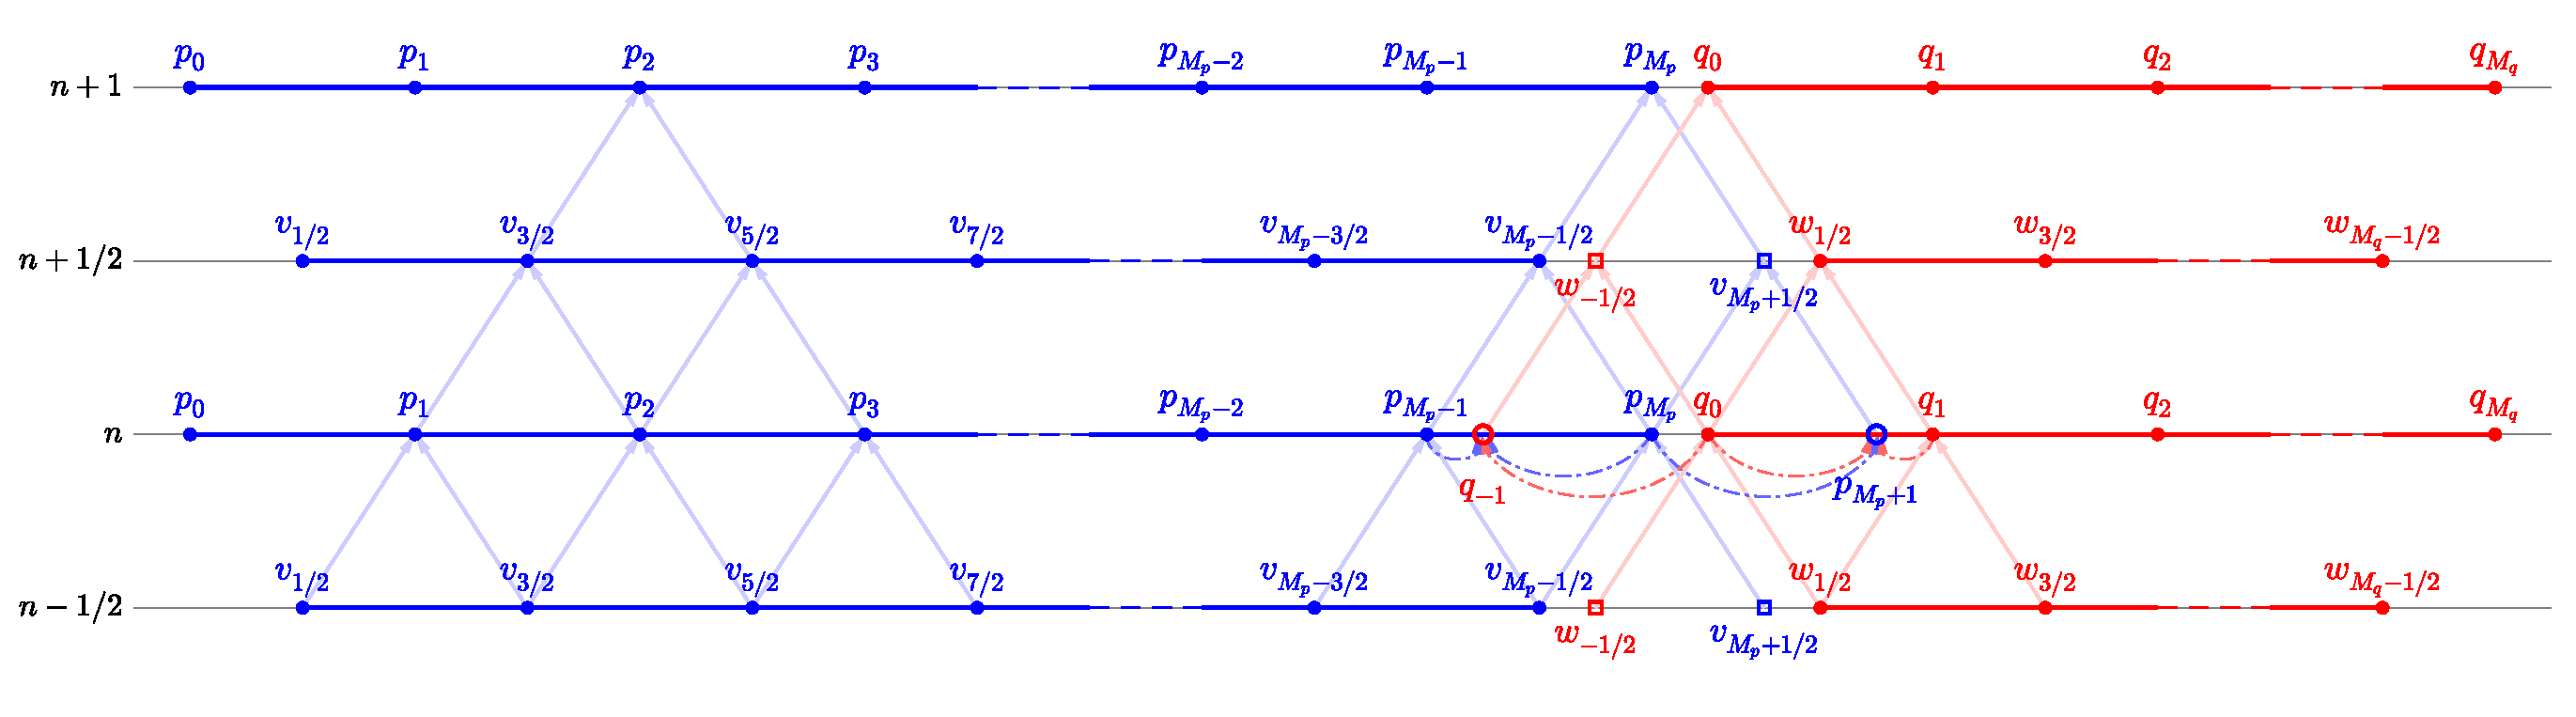
\includegraphics[width = \textwidth]{Figures/tromboneSchematic.eps}
    \caption{Schematic showing data flow of how different grid points at time index $n+1$ are calculated. To prevent cluttering, arrows going straight up (indicating that the state of a grid point at time step $n$ is needed to calculate the state of that grid point at $n+1$) are suppressed. As an example of the usual case, the points required to calculate $p_2^{n+1}$ are shown. Furthermore, the points needed to calculate $p_{M_p}^{n+1}$ and $q_0^{n+1}$ are shown. The most important difference with the usual case is that the virtual grid points $q_{-1}^n$ and $p_{M_p+1}^n$ are calculated from known values of $p^n$ and $q^n$ as opposed to values of $v^{n-1/2}$ and $w^{n-1/2}$.\label{fig:tromboneSchematic}}
\end{figure*}